\documentclass[a4paper,12pt,twoside]{report}

\usepackage{acronym}
\usepackage{url}
\usepackage{cite}
\usepackage{listings}
\usepackage[pdftex]{graphicx}
\usepackage[hang,small,bf]{caption}
\usepackage{styles/tum}
\usepackage{setspace}
\usepackage[german,english]{babel}
\usepackage{float}
\usepackage{floatflt}
\usepackage{fancyhdr}
\usepackage{color}
\usepackage{booktabs}
\usepackage[pdftex,bookmarks=true,plainpages=false,pdfpagelabels=true]{hyperref}
\usepackage{mdwlist}
\usepackage{enumerate}
\usepackage{paralist}
\usepackage{array}
\usepackage{longtable}
\usepackage{amsmath}
\usepackage{listings}
\usepackage[utf8]{inputenc}
\usepackage[capitalize, noabbrev]{cleveref}

% Path for graphics
\graphicspath{{figures/}}

\begin{document}
\setlength{\evensidemargin}{22pt}
\setlength{\oddsidemargin}{22pt}

\def\doctype{Bachelor's Thesis}
\def\faculty{Informatics}
\def\title{Simulation-Based Analysis of Blockchain Architectures}		
\def\titleGer{Simulationsbasierte Analyse von Blockchain Architekturen}
\def\supervisor{Broy, Manfred; Prof. Dr. rer. nat. habil.}
\def\advisor{Marmsoler, Diego; M.Sc.}
\def\author{Leo Eichhorn}
\def\date{15.07.2018}


\hypersetup{pdfborder={0 0 0},
                        pdfauthor={<author>},
                        pdftitle={<title english>},
                        }

\lstset{showspaces=false, numbers=left, frame=single, basicstyle=\small}

\pagenumbering{alph}

\thispagestyle{empty}

\vspace{4cm}
\begin{center}
\oTUM{4cm}\\ 
\vspace{5mm}     
\huge DEPARTMENT OF INFORMATICS\\ 
\vspace{0.5cm}
\large TECHNICAL UNIVERSITY OF MUNICH\\
\vspace{1mm}
\end{center}

\vspace{13mm}

\begin{center}
{\Large \doctype\ in \faculty}
\vspace{20mm}

\begin{spacing}{1.5}
{\huge\bf \title}\\%[3ex]
\end{spacing}

\vspace{15mm}
{\LARGE \author}

\vspace{10mm}

\begin{figure}[h!]
\centering
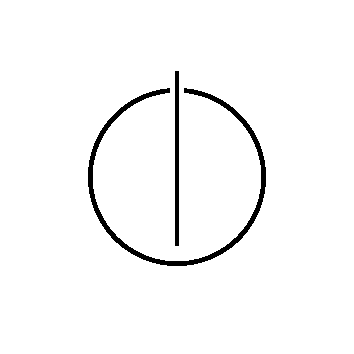
\includegraphics[width=4cm]{InformaticsLogo}
\end{figure}

\end{center}

\thispagestyle{empty}
\pagenumbering{roman}
\vspace{8mm}
\begin{center}
\oTUM{4cm}

\vspace{5mm}     
\huge DEPARTMENT OF INFORMATICS\\ 
\vspace{0.5cm}
\large TECHNICAL UNIVERSITY OF MUNICH\\
\end{center}

\vspace{5mm}

\begin{center}
{\Large \doctype\ in \faculty}
\vspace{8mm}

\begin{spacing}{1.3}
{\LARGE \title}\\
\vspace{8mm}

{\LARGE \titleGer}\\
\vspace{8mm}
\end{spacing}

\begin{tabular}{ll}
\Large Author:     & \Large \author     \\[2mm]
\Large Supervisor: & \Large \supervisor \\[2mm]				
\Large Advisor:	   & \Large \advisor    \\[2mm]
\Large Submission date:       & \Large \date
\end{tabular}

\vspace{1mm}

\begin{figure}[hb!]
\centering
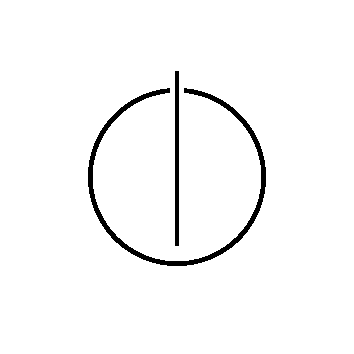
\includegraphics[width=4cm]{InformaticsLogo}
\end{figure}

\end{center}
\newpage
\thispagestyle{empty}
\mbox{}
\clearpage
\thispagestyle{empty}
\vspace*{0.8\textheight}
\noindent
I assure the single handed composition of this bachelor thesis only supported by declared resources,

\vspace{15mm}
\noindent
Munich, \date \hspace{\stretch{1}} \author
\newpage



\newpage
\thispagestyle{empty}
\mbox{}

\chapter*{Acknowledgements}


\pagenumbering{roman}

\selectlanguage{english}
\begin{abstract}

%abstract english

\textit{}

\end{abstract}

\clearpage

\selectlanguage{german}
\begin{abstract}

%abstract german
\textit{}

\end{abstract}

\clearpage

\selectlanguage{english}


\tableofcontents
\clearpage

\clearpage

\begin{acronym}
\acro{RADS}{Resistance of a blockchain architecture against double spend attacks}

\end{acronym}

\pagenumbering{arabic}

\fancyhead{}
\pagestyle{fancy}
\fancyhead[LE]{\slshape \leftmark}
\fancyhead[RO]{\slshape \rightmark}
\headheight=15pt




%------- chapter 1 -------

\chapter{Introduction}


%------- chapter 2 -------

\chapter{Background}
\section{Blockchain}
A blockchain is a public\footnote{In this thesis, only permissionless blockchains are considered, for permissioned blockchains see for example: \cite{p}}, distributed ledger used to record, identify and verify contracts, transactions or other shared data between multiple parties. These records are stored in a continuously growing list, which is locally maintained and updated by each individual member (node) of the protocol. Entries of the list (blocks) are cryptographically linked by including a hash of the previous block as a unique identifier in each newly added entry. More specifically, altering contents of a block changes its unique identifier, forcing a recalculation of every following block currently in the list, in order to retain integrity of the ledger. If consensus between nodes is reached through proof of work (Section \ref{pow}), consistently performing such an operation requires a substantial amount of computing power, arguably more than 50\% of the total computing power available to the whole Network. Newly created blocks are sent to all members to keep local blockchain copies synchronized. By adhering to a distributed consensus protocol, the participating nodes validate potential extensions of their blockchain copy in a peer-to-peer manner, thereby eliminating the need for an intermediary, trusted authority. 
 
\subsection{Applications}

\subsubsection{Cryptocurrencies}
\subsubsection{Smart Contracts}

\section{Bitcoin}
To improve our understanding of the blockchain technology and dynamics in a blockchain network we will now have a closer look at Bitcoin as a concrete example of a blockchain using proof of work 



\subsection{Transactions}


\subsection{Blocks}
\subsection{Proof of Work} \label{pow}
\subsection{Peer-to-peer Networks}

\section{Double-spend Attacks}

\section{Summary}
%------- chapter 3 -------

\chapter{Related Work}
\section{Hashrate-based Models for Double-Spend Attacks}
Potential attacks on blockchains, especially the Bitcoin protocol, have been conceptualized since the release of Nakamoto's original Bitcoin paper \cite{nakamoto2008bitcoin}. In chapter 11 of his proposal, Nakamoto formulates the first mathematical model to calculate the theoretical probability of successful double-spend attacks on his protocol. This model has since been improved and adapted several times, while similar, independent models have been formulated as well \cite{HBDSA,DSAwithTime,NakamotoDSACorrection,NakamotoExplMCSim}. Similar to \cite{DSAwithTime}, we will call the collection of these approaches \textit{hashrate-based} attack models. The central premise of a hashrate-based model is splitting the total computing power available to the network (hashrate \textit{H}), into two parts. To achieve this, \cite{HBDSA} defines \textit{pH} as the hashrate controlled by honest nodes adhering to the protocol, while \textit{qH} is used by malicious nodes trying to attack. Since also
\begin{subequations}
\renewcommand{\theequation}{\theparentequation.\arabic{equation}}
\begin{align}
p + q & = 1
\end{align}
\end{subequations}
it can easily be seen that \textit{p} and \textit{q} are precisely the probabilities of the next block being mined by either the honest or the attacking part of the network. Using an adaptation of the Gambler's Ruin problem \cite{gamblersruin}, Nakamoto and \cite{HBDSA} are now calculating the probability \textit{Q\textsubscript{z}} of an attacker successfully catching up with their fork of the blockchain, asuming they are at a total deficit of \textit{z} blocks compared to the honest nodes. The success of a potential double-spend attack against a merchant waiting for \textit{n} confirmations can now be formulated as the probability of \textit{Q\textsubscript{z}}, after \textit{n} blocks have been mined by the honest network. While \cite{nakamoto2008bitcoin} is using a poisson distribution in his formula, \cite{HBDSA} is achieving similar results with a negative binomial distribution. Combined with \cite{NakamotoDSACorrection}, the author of \cite{HBDSA} is also pointing out and correcting an of-by-one error introduced by Nakamoto, who is only calculating the probability of an attacker \textit{catching up} with his fraudulent blockchain fork, while for the double spend attack to be successful, the length of the honest chain has to be \textit{surpassed}. \cite{DSAwithTime} presents two similar approaches but considers partial advancement towards block creation as well. The author's first model extends the hashrate-based model formulated by \cite{HBDSA} and includes an additional parameter, indicating the time an attacker has already spent mining on blocks. The second model is fundamentally based on the time differences at which honest and attacking nodes have mined their last block, but is also relying on hashrates as a measure of computational power.
It is interesting to note that all of the before mentioned models produce similar results, despite the differences in their calculations. Therefore it is less surprising that the authors seem to agree on their general conclusions as well. Those can be summarized as follows:
\begin{itemize}
\item If an attacker controls the majority of computational power in the network, double-spend attacks will always succeed.
\item Probabilities for successful double-spend attacks decrease exponentially with an increasing number of confirmations.
\item Probabilities for successful double-spend attacks increase exponentially with an increasing amount of hashpower controlled by the attacker.
\item Although double-spend attacks at the standard of six confirmations are considered to be unlikely, there is nothing special about the number six.
\item Double-spend attacks are always possible, regardless of the number of confirmations and amount of computational power controlled by the attacker.
\end{itemize}
\section{Simulations}
An important remark can be seen in the fact that none of the before mentioned hashrate-based models have been confirmed by experimental data or tests in an exhaustive and realistic way. Instead, the validity of these models relies mostly on mathematical proofs and expertise, or the comparison with other, similar models. Nevertheless, one exception can be made with \cite{NakamotoExplMCSim}. After presenting a detailed explanation of Nakamoto's model for double-spends, the author validates the mathematical approach by performing a Monte Carlo simulation \cite{montecarlo} with different sets of input. In the light of this, the author identifies an error of the model, which is linked to its use of the poisson distribution. In spite of this success, the Monte Carlo simulation is missing parameters of a real blockchain protocol and ``does not actually
mine coin, it simply flips some coins to see whether each miner wins a block as simulated'' \cite{NakamotoExplMCSim}. Arguably important factors of blockchain dynamics, such as network propagation, mining difficulty and timing are disregarded. A more realistic simulation approach to a similar attack on Bitcoin blockchains is presented by \cite{mwalemodel}.
\section{Other Attacks}
\section{Contribution}
factor hidden behind ambiguous parameter hashrate
%------- chapter 4 -------

\chapter{Approach}

\section{Requirements}

\section{Overview}

\section{Design Goals}

\section{Subsystem Decomposition}


%------- chapter 5 -------

\chapter{Evaluation}

\section{Design}
	
\section{Objectives}

\section{Results}

\section{Findings}

\section{Discussion}

\section{Limitations}
\begin{itemize}
\item Scheduling
\item All attacking Nodes have equal, constant latency to each trusted node
\item Network creation not perfectly random

\end{itemize}

%------- chapter 6 -------

\chapter{Model}


%------- chapter 7 -------

\chapter{Summary}

\section{Status}

\subsection{Realized Goals}

\subsection{Open Goals}

\section{Conclusion}

\section{Future Work}


\appendix

\chapter{Source Code}


\clearpage

\listoffigures
\clearpage

\listoftables
\clearpage

\bibliography{thesis}
\bibliographystyle{alpha}

\end{document}
